\documentclass[dvipdfmx,11pt,notheorems]{beamer}
%%%% 和文用 %%%%%
\usepackage{bxdpx-beamer}
\usepackage{pxjahyper}
\usepackage{minijs}%和文用
\usepackage{listings,jlisting} % プログラムの表示用
\usepackage{type1cm}
\renewcommand{\kanjifamilydefault}{\gtdefault}%和文用

%%%% スライドの見た目 %%%%%
\usetheme{Boadilla}
\usecolortheme{seahorse}
\usefonttheme{professionalfonts}
\setbeamertemplate{frametitle}[default][center]
\setbeamertemplate{navigation symbols}{}
\setbeamercovered{transparent}%好みに応じてどうぞ)
\setbeamertemplate{footline}[page number]
\setbeamerfont{footline}{size=\normalsize,series=\bfseries}
\setbeamercolor{footline}{fg=black,bg=black}

\setbeamercolor{white-cyan1}
{fg=white,bg=cyan!80!black}
\setbeamercolor{white-cyan2}
{fg=white,bg=cyan!60!black}

%フラットデザイン化
\setbeamertemplate{blocks}[rounded] % Blockの影を消す
%Beamer色設定
\definecolor{UniBlue}{RGB}{0,150,200}
\definecolor{AlertOrange}{RGB}{255,76,0}
\definecolor{AlmostBlack}{RGB}{38,38,38}
\setbeamercolor{structure}{fg=UniBlue} % 見出しカラー
\setbeamercolor{block title}{fg=UniBlue!50!black} % ブロック部分タイトルカラー
%%%%

%%%% 定義環境 %%%%%
\usepackage{amsmath,amssymb}
\usepackage{amsthm}
\usepackage{bm}
\theoremstyle{definition}
\newtheorem{theorem}{定理}
\newtheorem{definition}{定義}
\newtheorem{proposition}{命題}
\newtheorem{lemma}{補題}
\newtheorem{corollary}{系}
\newtheorem{conjecture}{予想}
\newtheorem*{remark}{Remark}
\renewcommand{\proofname}{}
%%%%%%%%%

%%%%% フォント基本設定 %%%%%
% \usepackage[T1]{fontenc}%8bit フォント
% \usepackage{textcomp}%欧文フォントの追加
% \usepackage[utf8]{inputenc}%文字コードをUTF-8
% \usepackage{otf}%otfパッケージ
% \usepackage{lxfonts}%数式・英文ローマン体を Lxfont にする
% \usepackage{bm}%数式太字
%%%%%%%%%%

%%%%% 複数人の著者を揃える %%%%%
%% http://tex.stackexchange.com/questions/
%%   166531/how-to-change-author-alignment-in-beamer
\makeatletter
\long\def\beamer@author[#1]#2{%
  \def\insertauthor{\def\inst{\beamer@insttitle}\def\and{\beamer@andtitle}%
  \begin{tabular}{rl}#2\end{tabular}}%
  \def\beamer@shortauthor{#1}%
  \ifbeamer@autopdfinfo%
    \def\beamer@andstripped{}%
    \beamer@stripands#1 \and\relax
    {\let\inst=\@gobble\let\thanks=\@gobble\def\and{, }\hypersetup{pdfauthor={\beamer@andstripped}}}
  \fi%
}
\makeatother
%%%%%%%%%%

%%%%% プログラムに色をつける
\usepackage{color}

\definecolor{codegreen}{rgb}{0,0.6,0}
\definecolor{codegray}{rgb}{0.5,0.5,0.5}
\definecolor{codepurple}{rgb}{0.58,0,0.82}
\definecolor{backcolour}{rgb}{0.95,0.95,0.92}

\lstdefinestyle{mystyle}{
    backgroundcolor=\color{backcolour},
    commentstyle=\color{codegreen},
    keywordstyle=\color{magenta},
    numberstyle=\tiny\color{codegray},
    stringstyle=\color{codepurple},
    basicstyle=\footnotesize,
    breakatwhitespace=false,
    breaklines=true,
    captionpos=b,
    keepspaces=true,
    numbers=left,
    numbersep=5pt,
    showspaces=false,
    showstringspaces=false,
    showtabs=false,
    tabsize=2
}

\lstset{style=mystyle}

%%%%
\title[略タイトル]{第11回 知能システム学特論レポート}%[略タイトル]{タイトル}
\author[NishidaLab]{
15344203 & 有田 裕太 \\
15344206 & 緒形 裕太 \\
15344209 & 株丹 亮 \\
12104125 & 宮本 和 }%[略名前]{名前}
\institute[NishidaLab]{西田研究室,計算力学研究室}%[略所属]{所属}
\date{2015年\ 7月\ 27日}%日付

\begin{document}

%%%% 1 %%%%
\begin{frame}[plain]\frametitle{}
\titlepage %表紙
\end{frame}

% \begin{frame}\frametitle{Contents}
% \tableofcontents %目次
% \end{frame}

%%%% 進捗状況 %%%%
\begin{frame}\frametitle{進捗状況}

\begin{block}{理論研究の進捗}
畳込みニューラルネットワークの理論について
\end{block}

\vspace{1cm}
\begin{exampleblock}{プログラミングの進捗}
学習器のパラメータ設定について\\
アニメキャラクター認識時の中間層出力\\
データセットを作成し,学習を行った結果
\end{exampleblock}
\end{frame}

%%%%前回のグラフ%%%%
%\begin{frame}[fragile]\frametitle{学習結果}
% \begin{figure}[ht]
%  \centering
%  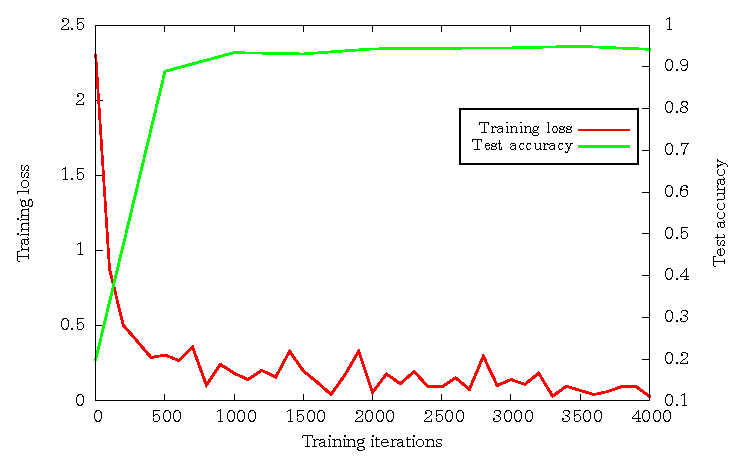
\includegraphics[scale=1.0]{fig/eps/result_train_test_graph.eps}
%  \caption{損失関数の値と精度 }
% \end{figure}
%\end{frame}



%%%%Dropout%%%%
\begin{frame}\frametitle{ドロップアウト}
 \begin{block}{ドロップアウト}
  多層ネットワークのユニットを確率的に選別して学習する方法
 \end{block}
 \begin{itemize}
  \item 自由度を下げて,過適合を避ける
  \item 複数のネットワークの平均をとり,精度が向上する
 \end{itemize}
\begin{figure}[tb]
  \begin{center}
    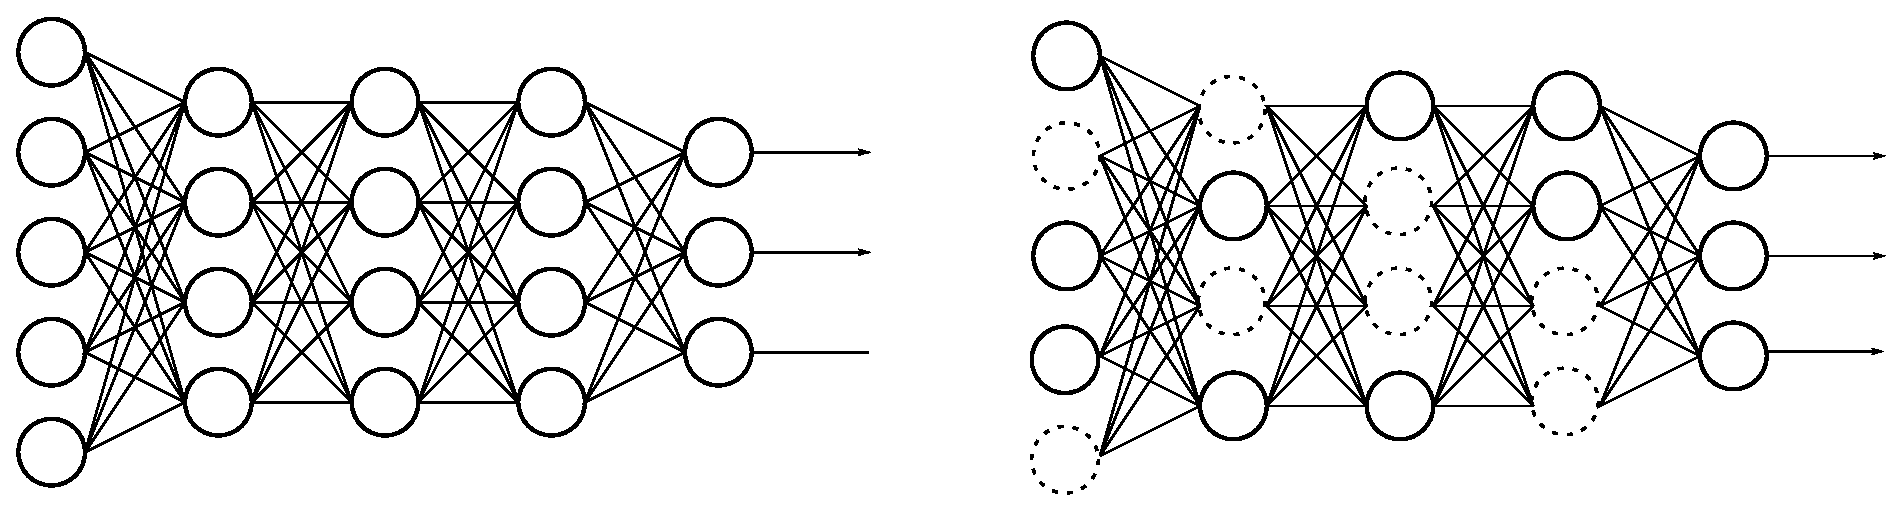
\includegraphics[clip,width=7cm]{./fig/eps/dropout1.eps}
  \end{center}
  \caption{ドロップアウト($p$=0.5程度)}
  \label{fig: ドロップアウト(p=0.5程度)}
\end{figure}
\vspace{-0.5cm}
 〜学習時〜
 \begin{itemize}
  \item 中間層の各層と入力層のユニットをある割合$p$でランダムに選出し,それ以外は無効化 $\rightarrow$ いつも通り最適化
 \end{itemize}
 〜学習終了後〜
 \begin{itemize}
  \item 無効化された層の出力を$p$倍し,すべてのユニットで逆伝播計算
 \end{itemize}
\end{frame}

%%%% 少女時代のメンバー識別でドロップアウトを試す %%%%
\begin{frame}\frametitle{Caffeでドロップアウトを試す}
\begin{itemize}
  \item 今まではアニメーション(ラブライブ!)を切り出して学習を行って,性能評価を行った.
  \item ラブライブ!のキャラクター識別は短い学習時間で高い学習精度を得ることができた.
  \item 学習の結果を解析したが,過学習の傾向は見られなかった.
  \item そこで次の課題として実在する人物の識別を行うことを目指し,韓国の女性アイドルグループ(少女時代)のメンバーの識別を試みた.
\end{itemize}
\begin{figure}[htbp]
  \begin{center}
    \includegraphics[clip,width=9cm,bb=0 0 1654 849]{./fig/jpg/snsd.jpg}
  \end{center}
\end{figure}

\end{frame}

%%%% 少女時代のメンバー識別でドロップアウトを試す %%%%
\begin{frame}[fragile]\frametitle{Caffeでドロップアウトを試す}
ラブライブ!の学習でも用いた通常のCifar10のモデルで学習を行った結果
\begin{figure}[tb]
  \begin{center}
    \includegraphics[clip,width=8cm]{./fig/eps/overtraining.eps}
  \end{center}
  \caption{通常のCifar10のモデルで実行した学習結果}
\end{figure}
\end{frame}

%%%% 少女時代のメンバー識別でドロップアウトを試す %%%%
\begin{frame}[fragile]\frametitle{Caffeでドロップアウトを試す}
\begin{alertblock}{結果}
訓練データに関しての精度は$1$に収束しているが,テストデータに関しては精度は$77\%$程度である.
\end{alertblock}
\begin{itemize}
  \item 理論に関する発表で説明したドロップアウトを導入し,過学習の回避を試みる.
  \item ドロップアウトのユニットを追加するだけでなく,\\過学習が起きる原因となる学習データの不足が考えられるため単純にデータセットを増やす以外の方法を模索.
  \item 入力として使うデータセットをランダムにクロップし入力データとして学習を行う方法と,入力データをランダムで左右反転させる方法
\end{itemize}
\end{frame}

%%%% 少女時代のメンバー識別でドロップアウトを試す %%%%
\begin{frame}[fragile]\frametitle{Caffeでドロップアウトを試す}
\begin{figure}[tb]
  \begin{center}
    \includegraphics[clip,width=8cm]{./fig/eps/dropout.eps}
  \end{center}
\end{figure}
\begin{block}{工夫の結果}
過学習を抑えることに成功.
最終的なテストデータに関する精度は$88\%$と通常のCifar10のモデルを使用した場合よりも精度向上が見られた.
\end{block}
\end{frame}

\begin{frame}\frametitle{アニメキャラクター認識時の中間層出力}
.prototexファイルを用いてキャラクター識別を行うため,$32\times 32$のサイ
ズに入力画像を変換する
\begin{figure}[t]
 \begin{minipage}{0.45\hsize}
  \centering
  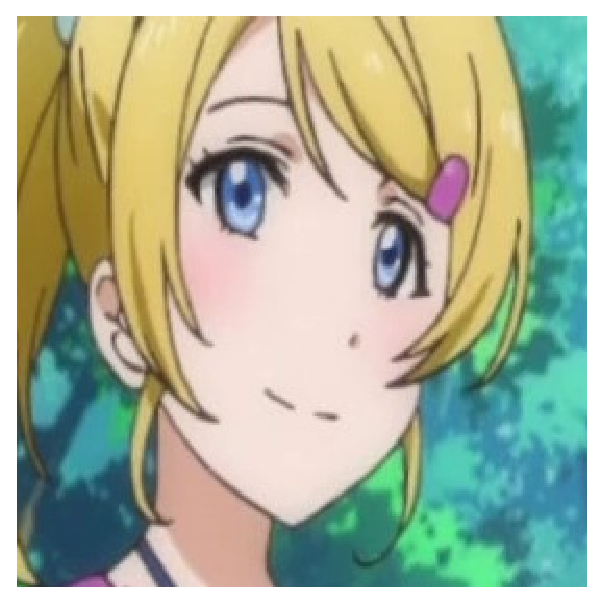
\includegraphics[width=50mm]{./fig/eps/eri.eps} \\
  \text{認識する画像}
 \end{minipage}
 \begin{minipage}{0.45\hsize}
  \centering
  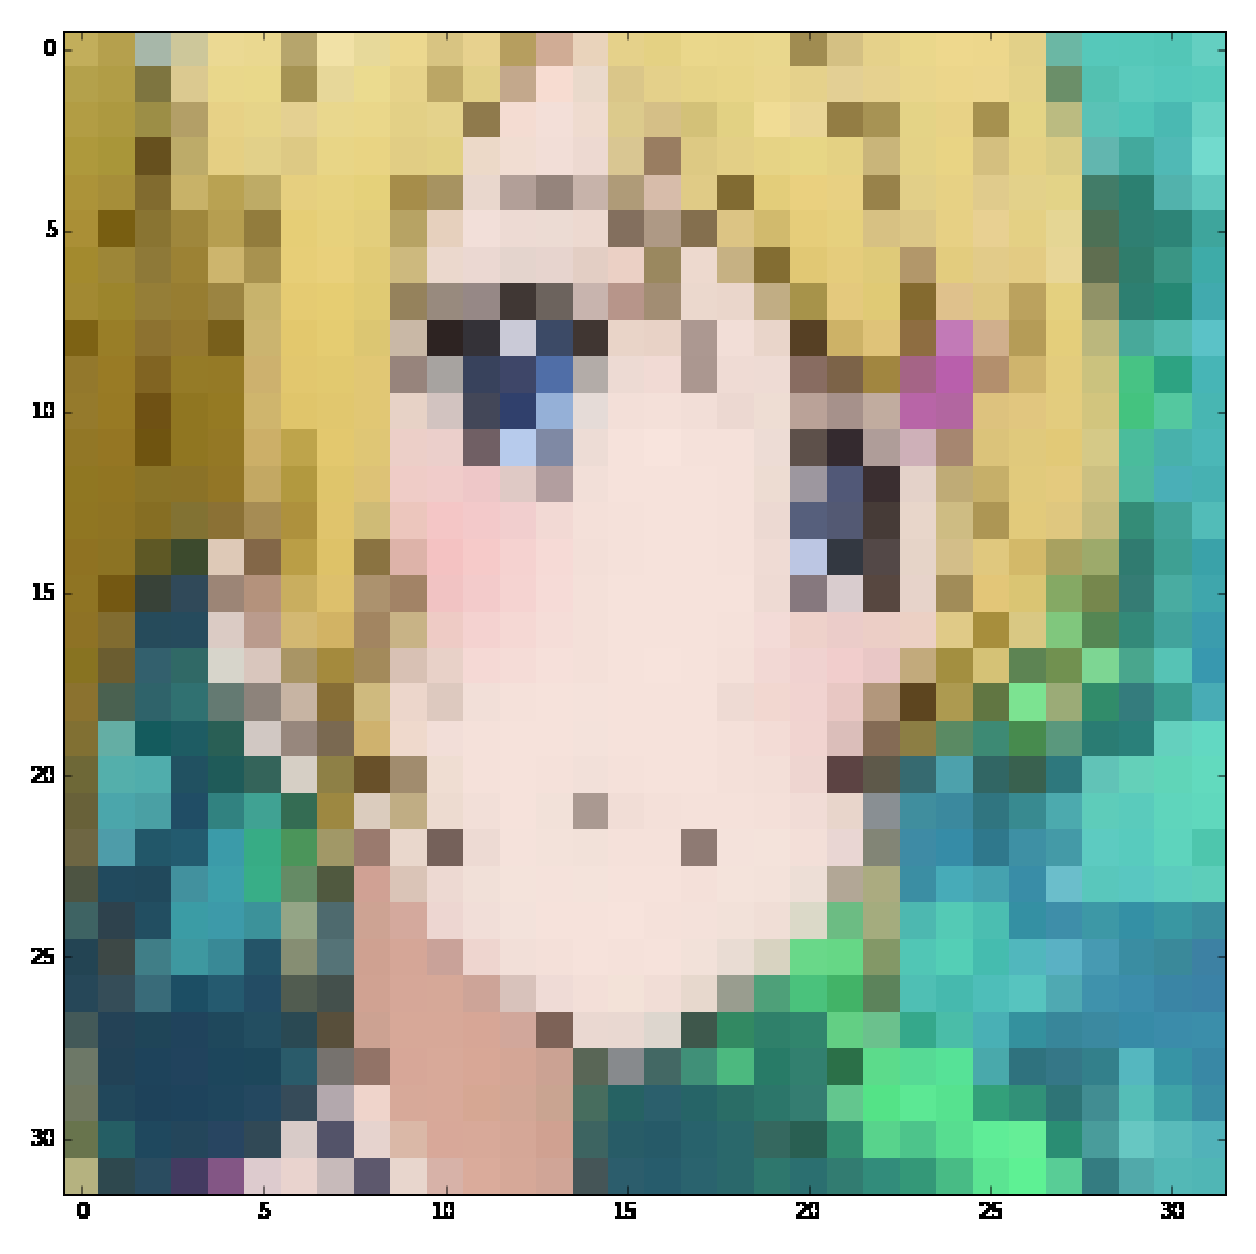
\includegraphics[width=50mm]{./fig/eps/inputeri.eps}\\
  \text{入力画像}
 \end{minipage}
\end{figure}

\end{frame}
\begin{frame}\frametitle{アニメキャラクター認識時の中間層出力}
\begin{figure}[t]
 \begin{minipage}{0.45\hsize}
  \centering
  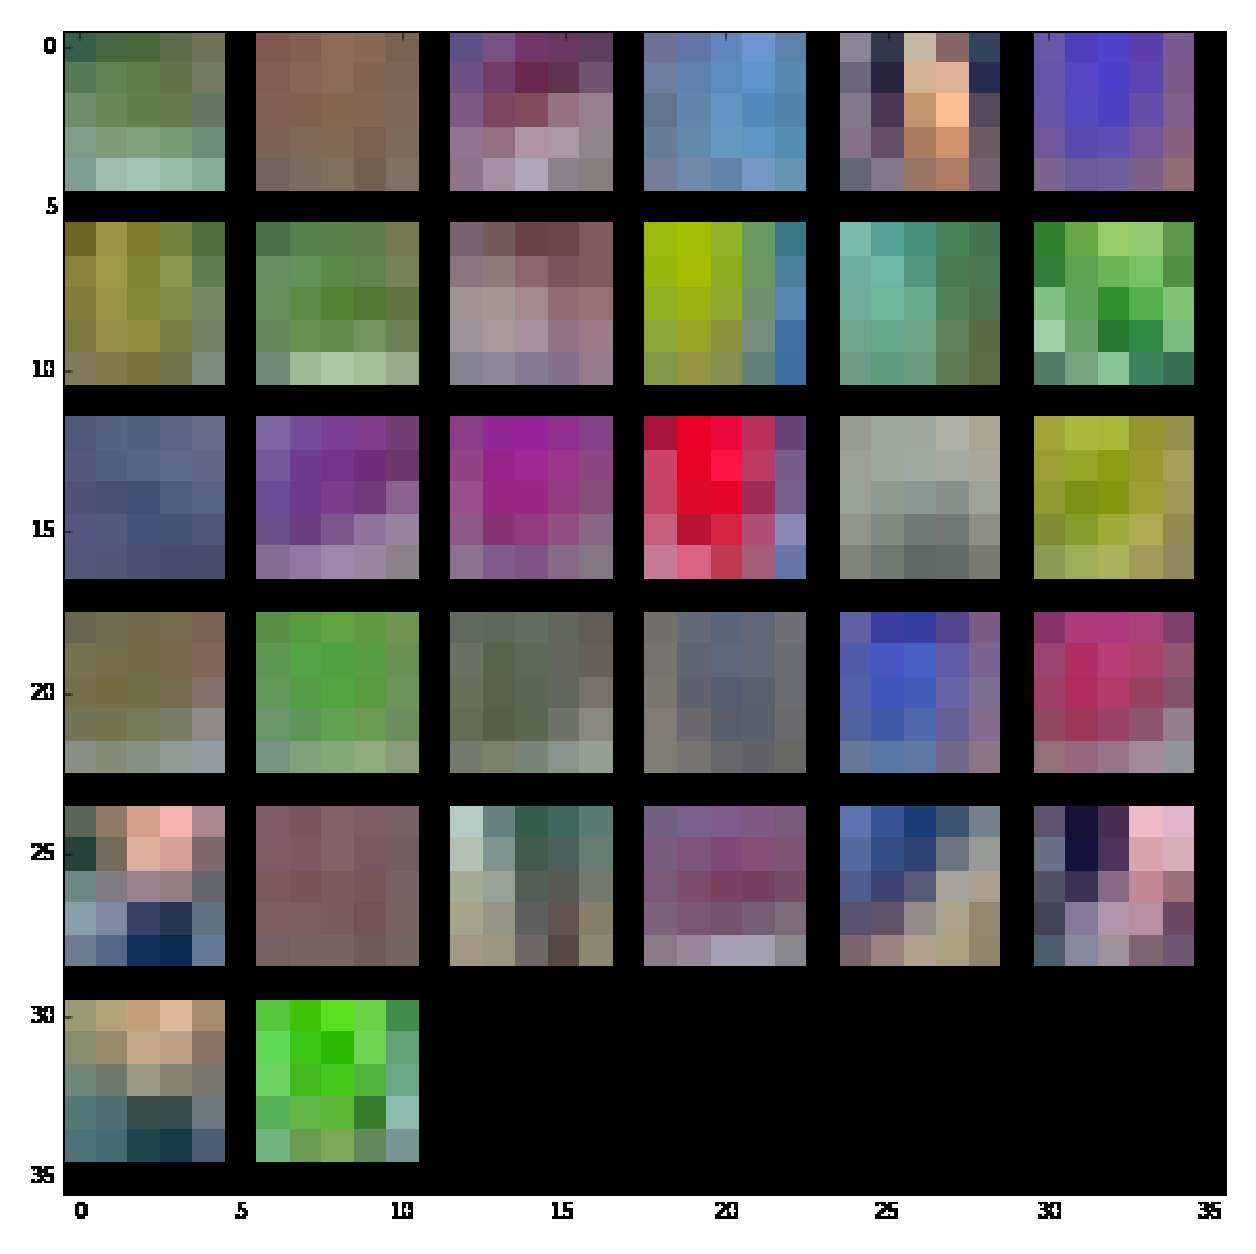
\includegraphics[width=50mm]{./fig/eps/filtereri.eps} \\
  \text{フィルタ}
 \end{minipage}
 \begin{minipage}{0.45\hsize}
  \centering
  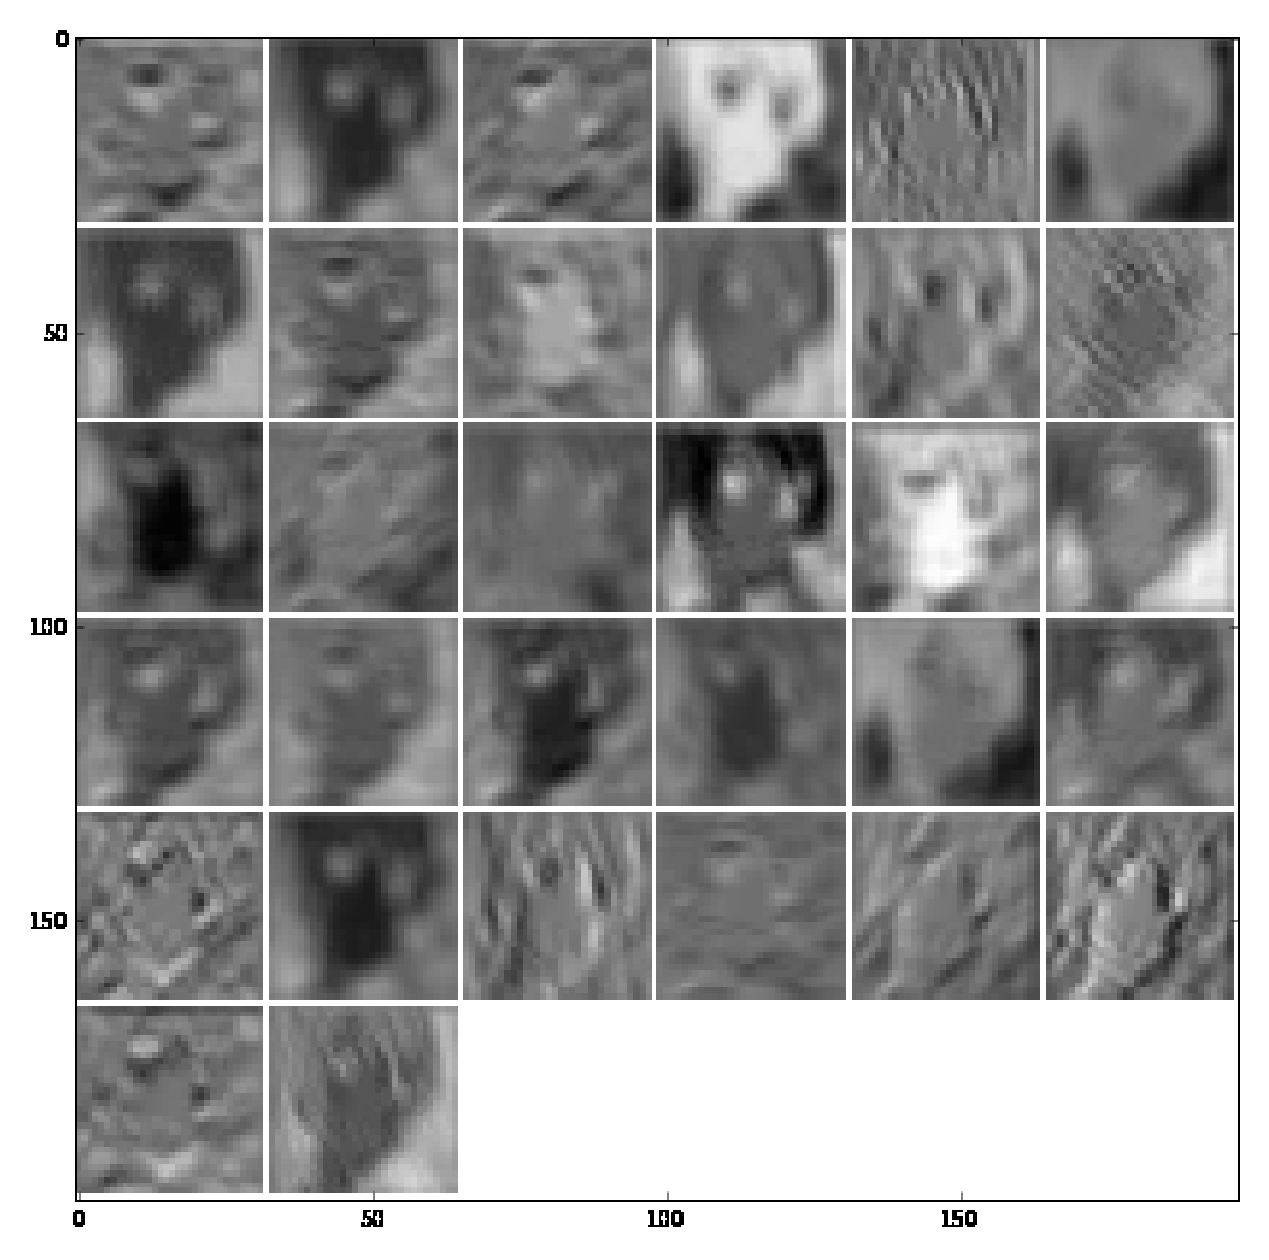
\includegraphics[width=50mm]{./fig/eps/outputeri.eps}\\
  \text{第一層目の出力}
 \end{minipage}
\end{figure}
\end{frame}

\begin{frame}\frametitle{学習データの強化}
\begin{figure}[t]
 \begin{minipage}{0.2\hsize}
  \centering
  \text{eri} \\
  \centering
  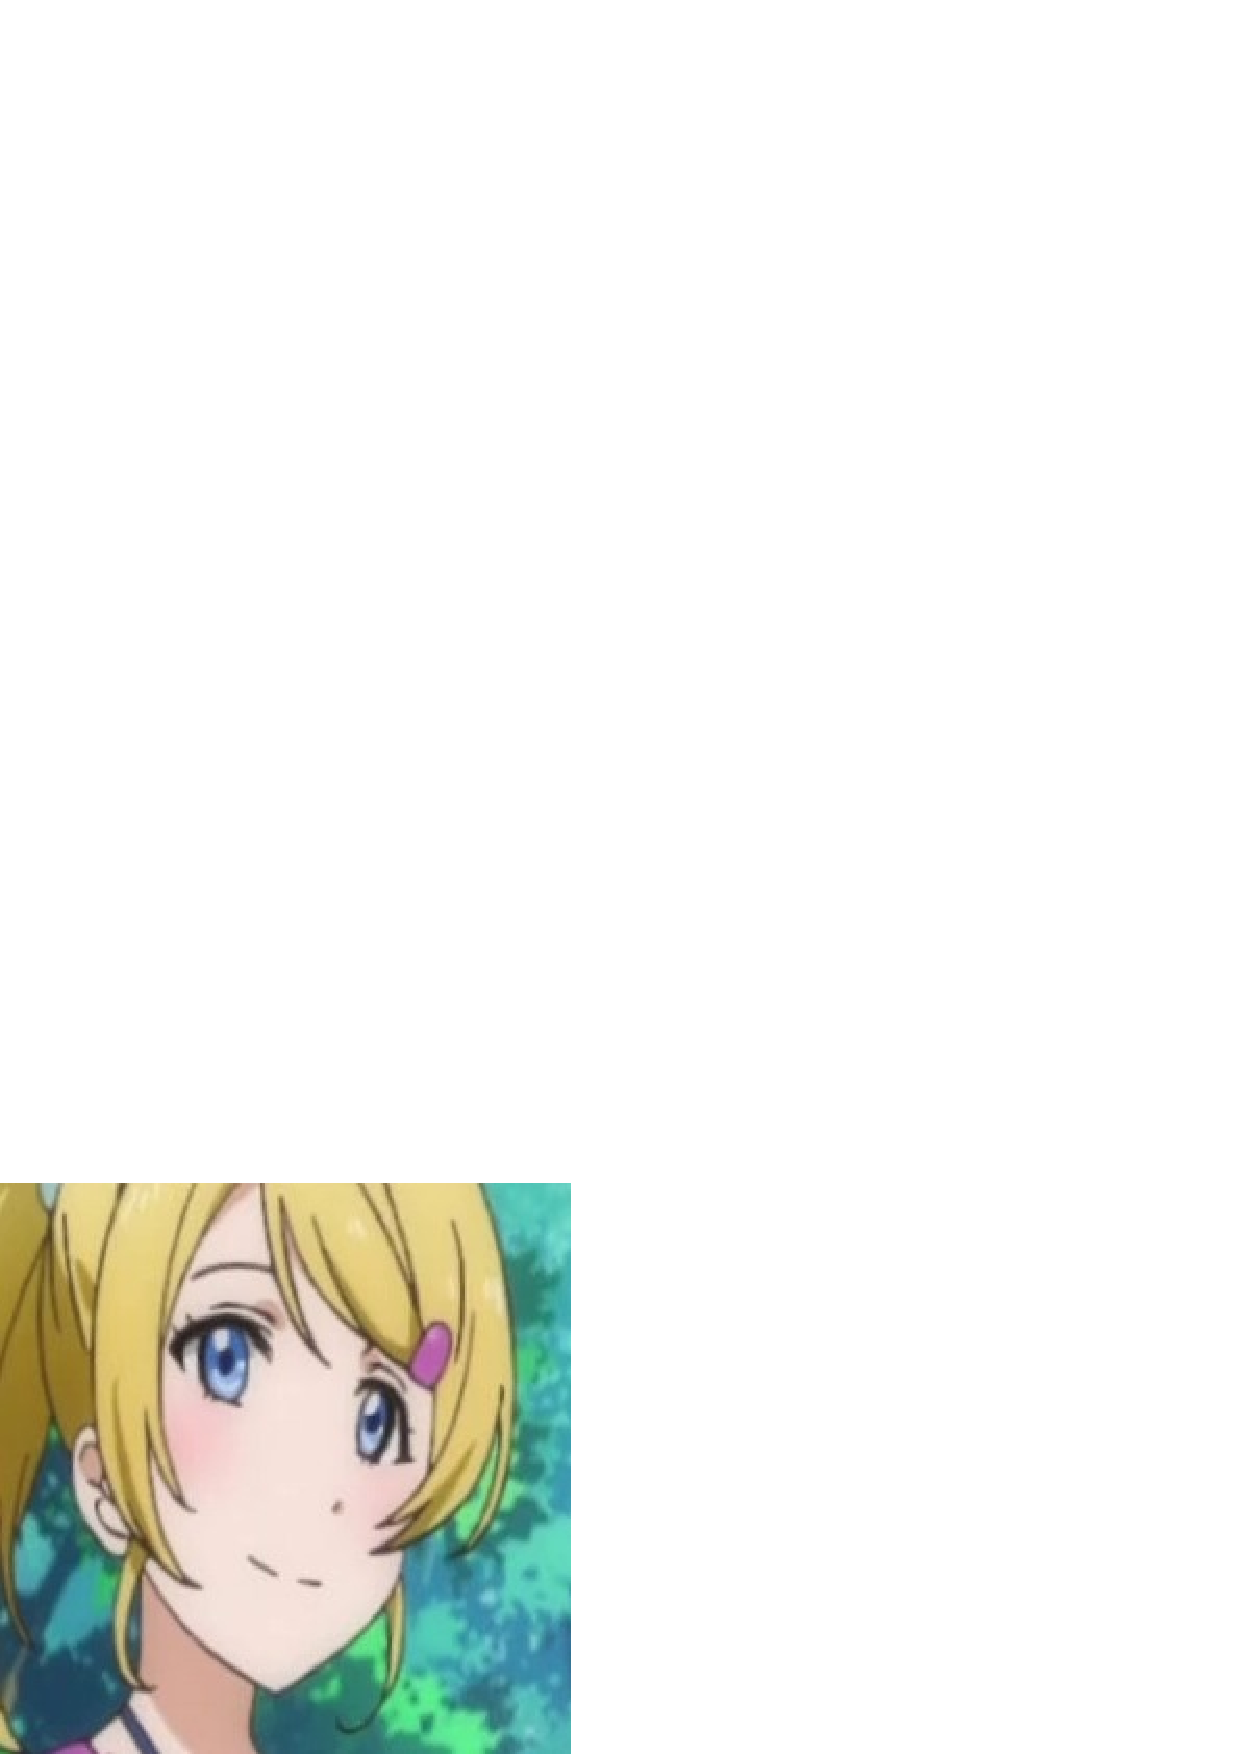
\includegraphics[width=20mm,bb=0 0 200 200]{./fig/png/faces/eri.png} \\
  \text{1908枚}\\
  \text{$\rightarrow$ 2816枚}
 \end{minipage}
 \begin{minipage}{0.2\hsize}
  \centering
  \text{hanayo} \\
  \centering
  \includegraphics[width=20mm,bb=0 0 200 200]{./fig/png/faces/hanayo.png}\\
  \text{2220枚}\\
  \text{$\rightarrow$ 3393枚}
 \end{minipage}
 \begin{minipage}{0.2\hsize}
  \centering
  \text{honoka} \\
  \centering
  \includegraphics[width=20mm,bb=0 0 200 200]{./fig/png/faces/honoka.png}\\
  \text{2733枚}\\
  \text{$\rightarrow$ 4176枚}
 \end{minipage}
 \begin{minipage}{0.2\hsize}
  \centering
  \text{kotori} \\
  \centering
  \includegraphics[width=20mm,bb=0 0 200 200]{./fig/png/faces/kotori.png}\\
  \text{1722枚}\\
  \text{$\rightarrow$ 2725枚}
 \end{minipage}
\end{figure}
\begin{figure}[t]
 \begin{minipage}{0.17\hsize}
  \centering
  \text{maki} \\
  \centering
  \includegraphics[width=20mm,bb=0 0 200 200]{./fig/png/faces/maki.png}\\
  \text{1874枚}\\
  \text{$\rightarrow$ 2768枚}
 \end{minipage}
 \begin{minipage}{0.17\hsize}
  \centering
  \text{niko} \\
  \centering
  \includegraphics[width=20mm,bb=0 0 200 200]{./fig/png/faces/niko.png}\\
  \text{1910枚}\\
  \text{$\rightarrow$ 3063枚}
 \end{minipage}
 \begin{minipage}{0.17\hsize}
  \centering
  \text{nozomi} \\
  \centering
  \includegraphics[width=20mm,bb=0 0 200 200]{./fig/png/faces/nozomi.png}\\
  \text{1489枚}\\
  \text{$\rightarrow$ 2144枚}
 \end{minipage}
 \begin{minipage}{0.17\hsize}
  \centering
  \text{rin} \\
  \centering
  \includegraphics[width=20mm,bb=0 0 200 200]{./fig/png/faces/rin.png} \\
  \text{2425枚}\\
  \text{$\rightarrow$ 3545枚}
 \end{minipage}
 \begin{minipage}{0.17\hsize}
  \centering
  \text{umi} \\
  \centering
  \includegraphics[width=20mm,bb=0 0 200 200]{./fig/png/faces/umi.png}\\
  \text{1703枚}\\
  \text{$\rightarrow$ 2409枚}
 \end{minipage}
 \end{figure}
負例(etc)7001枚$\rightarrow$9344枚
\end{frame}

\begin{frame}\frametitle{学習結果}
 \begin{figure}[ht]
 \centering
 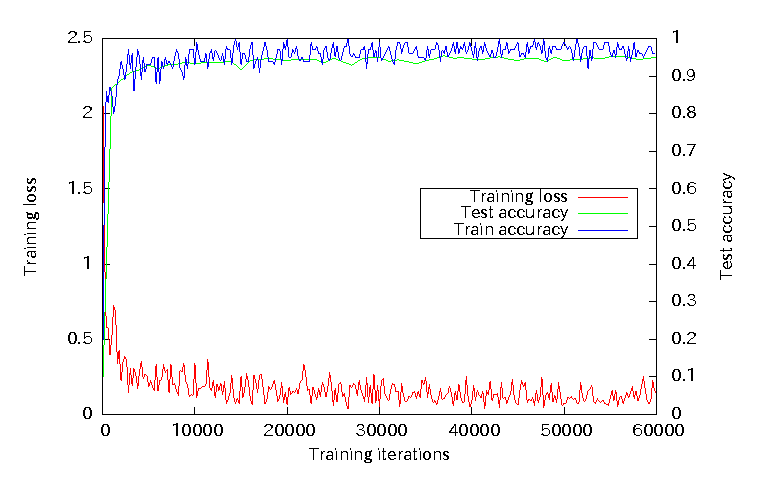
\includegraphics[scale=1.0]{fig/eps/result_train_test_lovelive_full.eps}
 \caption{損失関数の値と精度}
\end{figure}
\end{frame}

\begin{frame}\frametitle{識別結果の比較}
 \begin{figure}[t]
 \begin{minipage}{0.45\hsize}
  \centering
  \includegraphics[width=50mm]{./fig/jpg/lovelive-quick-result.jpg} \\
  \text{前回までの識別器を用いた}
  \text{識別結果}
 \end{minipage}
 \begin{minipage}{0.45\hsize}
  \centering
  \includegraphics[width=50mm]{./fig/jpg/lovelive-full-result.jpg}\\
  \text{データセットを増やした}
  \text{識別器を用いた識別結果}
 \end{minipage}
\end{figure}
\end{frame}

%%%% Caffeで識別 %%%%
% \begin{frame}\frametitle{caffeを使った識別}
% 前回の発表で説明した識別器を用いて実際に識別してみる.

% \begin{figure}[t]
%  \begin{minipage}{0.45\hsize}
%   \centering
%   \text{ラブライブ!} \\
%   \centering
%   \includegraphics[width=50mm]{./fig/jpg/lovelive.jpg} \\
%   \text{登録されている}
%   \text{アニメキャラクターの画像}
%  \end{minipage}
%  \begin{minipage}{0.45\hsize}
%   \centering
%   \text{アイドルマスター} \\
%   \centering
%   \includegraphics[width=50mm]{./fig/jpg/idolmaster.jpg}\\
%   \text{登録されていない}
%   \text{アニメキャラクターの画像}
%  \end{minipage}
% \end{figure}
% \end{frame}

% %%%% Caffeで識別結果1 %%%%
% \begin{frame}\frametitle{caffeを使った識別結果}

% \begin{figure}[t]
%   \centering
%   \text{ラブライブ!} \\
%   \centering
%   \includegraphics[width=100mm]{./fig/jpg/result_lovelive.jpg} \\
%   \text{登録されている}
%   \text{アニメキャラクターの画像}
% \end{figure}
% \end{frame}

% %%%% Caffeで識別結果2 %%%%
% \begin{frame}\frametitle{caffeを使った識別結果}

% \begin{figure}[t]
%   \centering
%   \text{アイドルマスター} \\
%   \centering
%   \includegraphics[width=100mm]{./fig/jpg/result_idolmaster.jpg} \\
%   \text{登録されていない}
%   \text{アニメキャラクターの画像}
% \end{figure}
% \end{frame}

% %%%% Caffeで識別結果3 %%%%
% \begin{frame}\frametitle{caffeを使った識別結果}

% \begin{figure}[t]
%   \centering
%   \text{真のラベルとの比較} \\
%   \centering
%   \includegraphics[width=100mm]{./fig/jpg/result_idol_compare.jpg} \\
%   \text{登録されていない}
%   \text{アニメキャラクターの画像}
% \end{figure}
% \end{frame}

%%%% 今後の課題 %%%%
\begin{frame}\frametitle{今後の課題}

\begin{block}{理論研究}
CNNの詳細な調査
\end{block}

\vspace{1cm}
\begin{exampleblock}{プログラミング}
学習画像を追加したり、パラメータを変更してみる
\end{exampleblock}
\end{frame}

% \begin{figure}[t]
%  \begin{minipage}{0.3\hsize}
%   \centering
%   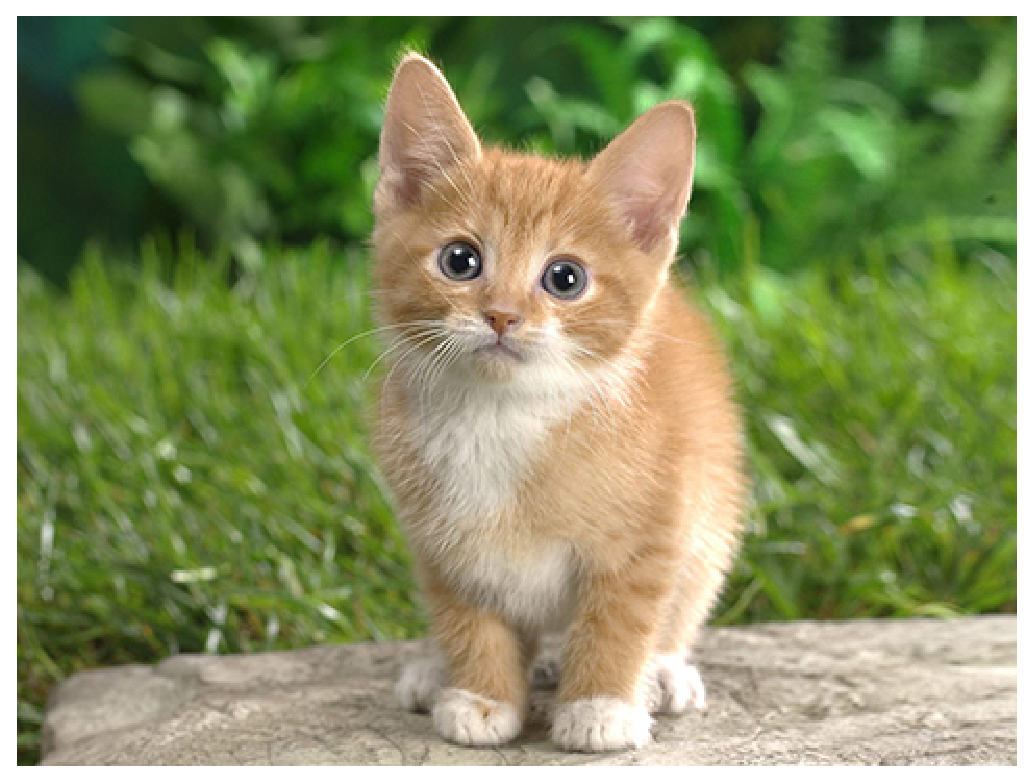
\includegraphics[width=30mm]{./figure/cat.eps}
%   \caption{cat.jpg}
%   \label{sample1}
%  \end{minipage}
%  \begin{minipage}{0.3\hsize}
%   \centering
%   \includegraphics[width=30mm]{./figure/cat_gray.eps}
%   \caption{cat\_gray.jpg}
%   \label{sample2}
%  \end{minipage}
%  \begin{minipage}{0.3\hsize}
%   \centering
%   \includegraphics[width=30mm]{./figure/fish-bike.eps}
%   \caption{fish-bike.jpg}
%   \label{sample3}
%  \end{minipage}
% \end{figure}
% \begin{exampleblock}{実行環境}
% \begin{itemize}
%  \item Ubuntu 14.04 LTS
%  \item Intel core i5-4440 3.10GHz$\times$4
%  \item RAM 16GB
% \end{itemize}
% \end{exampleblock}
% \end{frame}


% \section{具体例}

% \begin{frame}\frametitle{定理環境の例}
% \begin{theorem}[Fermat]
% $a^{p-1} \equiv 1 \pmod{p}$
% \end{theorem}
% \pause
% \begin{theorem}[Wilson]
% \begin{equation}
% (p-1)! \equiv 1 \pmod{p}
% \end{equation}
% \end{theorem}
% \end{frame}

% \begin{frame}<1-2>\frametitle{オーバーレイ}
% \onslide*<1>{
% \Large{これは1枚目です}
% }
% \onslide*<2>{
% これは2枚目です
% \begin{theorem}[Euclid]
% There is no largest prime number.
% \end{theorem}
% }
% \end{frame}

% \begin{frame}\frametitle{色もつけれるよ}
%   {\color{red} red}(\alert{alert}),
%   {\color{blue} blue}(\structure{structure}),
%   {\color{green} green},
%   {\color{cyan} cyan},
%   {\color{magenta} magenta},
%   {\color{yellow} yellow},
%   {\color{black} black},
%   {\color{darkgray} darkgray},
%   {\color{gray} gray},
%   {\color{lightgray} lightgray},
%   {\color{orange} orange},
%   {\color{violet} violet},
%   {\color{purple} purple},
%   {\color{brown} brown},
% \end{frame}

% \begin{frame}\frametitle{いろんなブロック}
% \begin{block}{ブロック}
% これは普通のブロックです
% \end{block}

% \begin{alertblock}{警告ブロック}
% 警告!これは警告ブロックだ!
% \end{alertblock}

% \begin{exampleblock}{例ブロック}
% 例えば、こんなブロックです。
% \end{exampleblock}
% \end{frame}

% \begin{frame}<1-2>\frametitle{画像も貼れるよ}
% \onslide*<1>{
% このように画像を貼れるよ
% %\begin{figure}[htb]
% %\centering
% %\includegraphics[width=12cm,clip]{dummygraph.pdf}
% %\caption{$f(x)=e^{-\frac{x}{10}}\sin(x)$}
% %\end{figure}%
% }
% \onslide*<2>{
% 画像や表は各自用意してね
% %\begin{figure}[htb]
% %\centering
% %\includegraphics[width=8cm,clip]{sym4.pdf}
% %\caption{Cayley graph of $\mathfrak{S}_{4}$}
% %\end{figure}%
% }
% \end{frame}

% \begin{frame}\frametitle{まとめ}
% \LARGE{大事なのは中身です!}
% \end{frame}

% \begin{frame}\frametitle{}
% {\Large ありがとうございました}
% \end{frame}
% \appendix

\newcounter{finalframe}
\setcounter{finalframe}{\value{framenumber}}

% \begin{frame}[containsverbatim]\frametitle{dvipngの使い方(1)}
% \begin{block}{この様なファイルを用意する}
% \tiny{
% \begin{verbatim*}
% \documentclass[43pt]{jsarticle}
% \usepackage{amsmath}
% \usepackage{lmodern}
% \pagestyle{empty}
% \begin{document}
% \begin{equation*}
% \sum_{k=0}^{\infty} \frac{(2k)!}{2^{2k}(k!)^2} \frac{1}{2k+1}=\frac{\pi}{2}
% \end{equation*}
% \end{document}
% \end{verbatim*}
% }
% \end{block}
% \end{frame}

% \begin{frame}[containsverbatim]\frametitle{dvipngの使い方(2)}
% \begin{block}{使い方(コマンドライン)}
% \scriptsize{
% \begin{verbatim*}
% latex dvipng-sample.tex
% dvipng dvipng-sample.dvi -T tight -bd 1000
% \end{verbatim*}
% }
% \end{block}
% \end{frame}
\setcounter{framenumber}{\value{finalframe}}
\end{document}